\renewcommand{\thefigure}{\Asbuk{section}.\arabic{figure}}
\renewcommand{\thetable}{\Asbuk{section}.\arabic{table}}
\renewcommand{\thelstlisting}{\Asbuk{section}.\arabic{lstlisting}}

\chead{\vspace{1ex}Продолжение приложения А}
\pagestyle{fancy}
\thispagestyle{plain}

\begin{landscape}
\section*{ПРИЛОЖЕНИЕ A\\(справочное)\\<название приложения>\\(к подразделу <номер подраздела>)}

\setcounter{section}{1}
\setcounter{figure}{0}
\setcounter{table}{0}
\setcounter{lstlisting}{0}

В редких случаях бывает удобно выделять объемные рисунки и таблицы, а также листиниги в приложения:

\begin{figure}[h]
\centering
  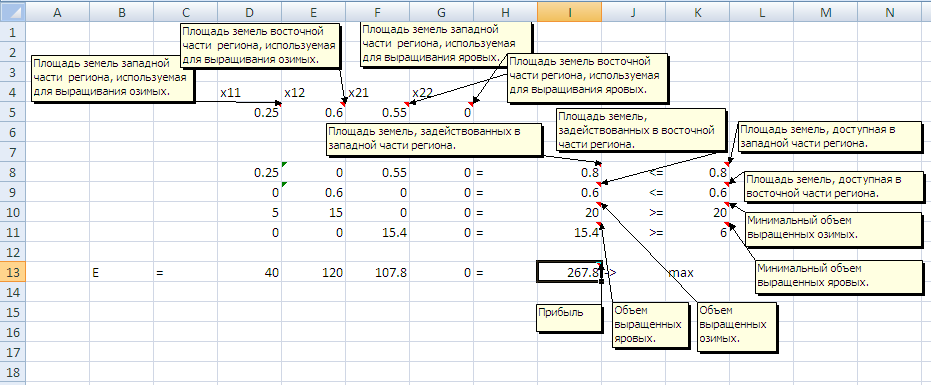
\includegraphics[width=0.8\linewidth]{fig/excel}
  \caption{Рабочий лист Excel с результатами решения базовой задачи линейного программирования}
\end{figure}

\end{landscape}

\newpage
